%!TEX ROOT=formularioFisica.tex

\section{Magnetismo}\label{sec:magnetismo}
Il magnetismo si occupa di come i magneti interagiscano fra di loro. Ogni magnete genera un
campo magnetico ($\vec{B}$). La sua direzione � sempre dal polo NORD a quello SUD. Ogni magnete ha
sempre due poli e anche se lo si divide si otterranno magneti bipolari.\\ 
La sua unit� di misura � il \emph{Tesla} ($T = \frac{N}{Am}$)\\
Pu� essere definito in due modi, prenderemo in considerazione quello pi� usato in ambito liceale.\\
Per gli esercizi si vada \hyperref[ex:magnetismo]{qui}.

\subsection{Forza in un campo magnetico}
\begin{equation*}	
\vec{F} = l\cdot(\vec{i}\times\vec{B})
\end{equation*}
Si ricordi che questo � un \hyperref[subsec:vettori:prodottoVettoriale]{prodotto vettoriale}.\\
$l$ rappresenta la lunghezza del cavo che attraversa il campo magnetico\\
$\vec{i}$: � la corrente che attraversa il cavo. IL verso determiner� se da considerarsi positiva o
negativa nel sistema di riferimento scelto.

\subsection{Legge di Biot-Savant}
La legge di Biot-Savant definisce un campo magnetico generato da un filo rettilineo percorso da
una corrente.\\
La direzione � la tangente alla linea di forza generata dal filo, il verso � antiorario se la
corrente esce, orario altrimenti. Un modo per ricordarselo pi� facilmente � il seguente: si prenda la
mano destra e si usi il pollice per indicare il verso e la direzione della corrente. Si chiudano poi
a pugno le altre dita. Il verso delle dita chiuse, � anche quello del campo magnetico.
\begin{equation*}
B = \frac{\mu_0}{2\pi}\frac{i}{d}
\end{equation*}
\hyperref[tab:mu0]{$\mu_0$}: $4\pi\cdot10^{-7}\,\text{N/A}^2$\\
\hyperref[tab:pi]{$\pi$}: $3.14$\\
$i$: corrente\\
$d$: distanza dal filo\\

\subsection{Legge di Amp�re}
La legge di Amp�re descrive la forza che intercorre tra due fili paralleli attraversati da una
corrente.
\begin{equation*}
F = \frac{\mu_0}{2\pi}\frac{i_1i_2}{d}l
\end{equation*}
\hyperref[tab:mu0]{$\mu_0$}: $4\pi\cdot10^{-7}\,\text{N/A}^2$\\
\hyperref[tab:pi]{$\pi$}: $3.14$\\
$i$: corrente\\
$d$: distanza tra i due fili\\[\baselineskip]
Molto spesso si vuole definire la forza su di una certa dimensione del filo, quindi si ottiene
la formula in questa forma:
\begin{equation*}
\frac{F}{l} = \frac{\mu_0}{2\pi}\frac{i_1i_2}{d}l
\end{equation*}
La formula calcola il modulo del vettore. La forza � attrattiva se i versi delle correnti sono 
uguali, repulsiva altrimenti.

\subsection{Motore elettrico}
Nonostante il nome possa far credere che funziona solo attraverso l'elettricit�, il motore elettrico 
svolge la sua funzione grazie ad una coesione di elettricit� e magnetismo. Il disegno seguente 
cercher� di chiarire le idee.
\begin{center}
	\begin{tikzpicture}
		% Magnets
		\coordinate (N1) at (0,1);
		\coordinate (N2) at (0,-1);
		\coordinate (S1) at (3,1);
		\coordinate (S2) at (3,-1);
		% Plate
		\coordinate (P1) at (1,0.5);
		\coordinate (P2) at (2,-0.5);
		
		% Magnets
		\draw[thick] (-0.5,1) -- (N1) -- (N2) -- (-0.5,-1);
		\draw[thick] (3.5,1) -- (S1) -- (S2) -- (3.5,-1);
		% Plate
		\draw[thick] (P1) -- (P2);
		
		% Magnetic lines
		\foreach \a in {0.8,0,-0.8}{
			\draw[gray, very thin, -stealth] (0.2, \a) -- ++(2.6,0);
		}
		
		\draw[-stealth] (P1) -- ++(0,0.7);
		\draw[-stealth] (P2) -- ++(0,-0.7);
		
		% Annotations
		\node at (-0.5,0){$N$};
		\node at (3.5,0){$S$};
		\node at (1.7,0.3){$P$};
		\node at (0.5,-1.2){$\vec{B}$};
		\node at ($(P1)+(0,0.9)$){$\vec{F}$};
		\node at ($(P2)+(0,-0.9)$){$\vec{F}$};
	\end{tikzpicture}
\end{center}
Come funziona? Innanzitutto abbiamo un campo magnetico $N-S$ e una spira rettangolare $P$ attraverso 
la quale passa corrente (solitamente � caratterizzata da un vasto numero di strati). Si fa passare 
corrente all'interno di questa spira in modo che una forza si generi. Questa forza metter� in 
rotazione la spira. Quando si raggiunge la situazione in cui il momento � $0$ (ovvero quando � 
perpendicolare al campo) la corrente viene invertita cos� che la piastra continui il giro. Questa 
forza motrice � quella che si genera e verr� poi usata.\\
Per capire meglio il movimento si guardi il disegno qua sotto
\begin{center}
	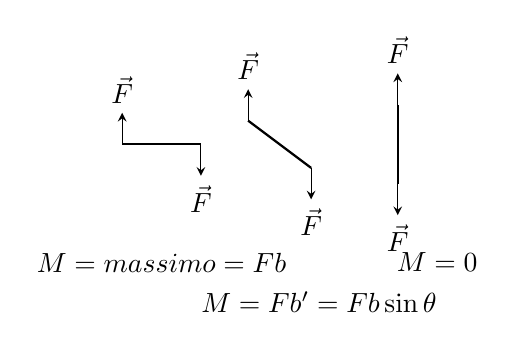
\begin{tikzpicture}
		\coordinate (P1) at (0,0);
		\coordinate (P2) at (1,0);
		
		\coordinate (P3) at (1.6,0.3);
		\coordinate (P4) at (2.4,-0.3);
		
		\coordinate (P5) at (3.5,0.5);
		\coordinate (P6) at (3.5,-0.5);
		
		\draw[thick] (P1) -- (P2);
		\draw[thick] (P3) -- (P4);
		\draw[thick] (P5) -- (P6);
		
		\draw[-stealth] (P1) -- ++(0,0.4)
			node[pos=1,above]{$\vec{F}$};
		\draw[-stealth] (P2) -- ++(0,-0.4)
			node[pos=1,below]{$\vec{F}$};
			
		\draw[-stealth] (P3) -- ++(0,0.4)
			node[pos=1,above]{$\vec{F}$};
		\draw[-stealth] (P4) -- ++(0,-0.4)
			node[pos=1,below]{$\vec{F}$};
			
		\draw[-stealth] (P5) -- ++(0,0.4)
			node[pos=1,above]{$\vec{F}$};
		\draw[-stealth] (P6) -- ++(0,-0.4)
			node[pos=1,below]{$\vec{F}$};
			
		\node at (0.5,-1.5){$M =\text{ massimo} = Fb$};
		\node at (2.5,-2){$M=Fb'=Fb\sin\theta$};
		\node at (4,-1.5){$M=0$};
	\end{tikzpicture}
\end{center}

\subsection{Forza di Lorenz}
La forza di Lorenz � la forza che una carica in moto risente all'interno di un campo magnetico.
\begin{equation*}
\vec{F} = q\vec{v}\times\vec{B}
\end{equation*}

Si presti attenzione al verso di questa forza. Se la carica � \emph{positiva} si usi la solita
regola della mano, altrimenti si inverta semplicemente il verso.\\[\baselineskip]	
Una particolarit� � che una carica che entra in un campo magnetico viene deviata dal suo percorso.
Il moto che ne deriva � \emph{elicoidale}. Ovviamente questo nel caso pi� generale, il disegno
di seguito aiuter� a capire in che modo l'elettrone viene spostato

\begin{center} % https://tex.stackexchange.com/questions/129860/helix-on-a-cylinder
	\tdplotsetmaincoords{70}{15}
	\begin{tikzpicture}[tdplot_main_coords]
	
		% --- Independent parameters ---
		\def\h{3}                          % cylinder height
		\pgfmathtruncatemacro\tA{350}      % A angle
		\def\zA{1}                         % A applicate
		\pgfmathtruncatemacro\tB{150}      % B angle
		\def\zB{2}                         % B applicate
		\pgfmathtruncatemacro\n{3}         % number of additional turns
		\pgfmathtruncatemacro\NbPt{100}    % number of dots for drawing the helix portion
		\def\rhelixdots{0.05}              % radius of dots forming helix
		\def\rAB{0.05}                     % radius of A and B dots
		
		% lower circle
		\draw[black,very thin] (1,0,0) 
		\foreach \t in {2,3,...,360}
		{
			--({cos(\t)},{sin(\t)},0)
		}
		--cycle;
		
		% upper circle
		\draw[black,very thin] (1,0,\h) 
		\foreach \t in {2,4,...,360}
		{
			--({cos(\t)},{sin(\t)},\h)
		}
		--cycle;
		
		% --- Draw helix ---
		\pgfmathsetmacro\tone{\tA}
		\pgfmathsetmacro\tlast{\tB+\n*360}
		\pgfmathsetmacro\ttwo{\tone+(\tlast-\tone)/(\NbPt-1)}
		\pgfmathsetmacro\p{360*(\zB-\zA)/(\tB-\tA+360*\n)}
		\foreach \t in {\tone,\ttwo,...,\tlast}{%
			\fill[red!80] ({cos(\t)},{sin(\t)},{\p*(\t-\tA)/360+\zA}) circle[radius=\rhelixdots];
		}
		
		% --- Draw A and B ---
		\fill[blue] ({cos(\tA)},{sin(\tA)},\zA) circle [radius=\rAB]node[right]{$A$};
		\fill[blue] ({cos(\tB)},{sin(\tB)},\zB) circle [radius=\rAB]node[left]{$B$};
	\end{tikzpicture}
\end{center}
Questa � una rappresentazione del moto di una carica all'interno del campo magnetico. Queste formule
permettono di trovare il \emph{raggio}, \emph{periodo} e il \emph{passo} dell'elica.
\begin{alignat*}{2}
r &= \frac{m\cdot v}{q\cdot B} &\qquad  T &= \frac{m\cdot v_x}{q\cdot B}\\
\delta S &= v_y = T &\qquad F &= m\frac{v^2}{r}
\end{alignat*}
Queste formule sono state ottenute equivalendo la forza di Lorenz e quella centripeta in quanto abbiamo
comunque un modo circolare.
Sempre supposto che $\vec{B}\perp\vec{v}$, il periodo si pu� scrivere anche come
\begin{equation*}
T = \frac{2\pi\cdot m}{q\cdot B}
\end{equation*}

\subsection{Selettore di velocit�}
Il selettore di velocit� � un particolare dispositivo che permette di "selezionare" alcune cariche che
vanno solo ad una determinata velocit� attraverso una fessura. Il loro utilizzo � molto ampio, 
specialmente in dispositivi come televisioni a tubo catodico.\\
Il loro funzionamento si basa su due campi $\vec{E}$ e $\vec{B}$ uniformi incrociati fra di loro.\\
Sulla carica deve agire una forza $\vec{F}$ pari a
\begin{equation*}
\vec{F} = q\vec{E} + q\vec{v}\times\vec{B}
\end{equation*}
Una carica passa nel selettore se e solo se la sua velocit� � pari a
\begin{equation*}
v = \frac{E}{B}
\end{equation*}

\subsection{Conduttori nei metalli}
In questa sottosezione si trovano le formule per trovare la carica massima che pu� ottenere e la
velocit� di deriva degli elettroni.\\

\subsubsection{Carica massima}
\begin{equation*}
i = n\cdot A\cdot v_d\cdot e
\end{equation*}
\hyperref[tab:e-]{$e$}\\
$n$: numero di elettroni di conduzione77
$A$: sezione del conduttore

\subsubsection{Velocit� di deriva}
\begin{equation*}
v_d = \frac{i}{n\cdot A\cdot e}
\end{equation*}
\hyperref[tab:e-]{$e$}\\
$n$: numero di elettroni di conduzione77
$A$: sezione del conduttore